\chapter{Data Analysis}

\MyQuote{In physics, you don't have to go around making trouble for yourself - nature
does it for you.}{Frank Wilczek}

QCD jets are the most common hard objects observed in the ultrarelativistic
collisions at hadron colliders, with their cross section exceeding any other
physics process by orders of magnitude.  Measurement of inclusive jet cross
section thus provides the test for both QCD predictions and the detector
performance up to the momentum transfers not reachable by any other physics
processes. 

This chapter describes the details of the double differential inclusive jet
cross section analysis.

\section{Data Characteristics}

Data used in this thesis are Monte Carlo generated events of $pp$ collisions at
the center-of-mass energy $\sqrt{s} = 13\TeV$ with \textsc{Pythia8}
\cite{Pythia8} event generator using CT10 PDFs \cite{CT10PDF} and ATLAS underlying event
tune AU2 \cite{AU2}. QCD calculations are done only to the leading order in
\textsc{Pythia8}. The response of the ATLAS detector on these events was
calculated with \textsc{Geant4} \cite{Geant4} software toolkit.

Particles were recombined into jets using anti-$k_t$ jet algorithm with parameter $R=0.4$.
There are particle jets reconstructed from the \textsc{Pythia8} output, which
further in this thesis are denoted truth jets, and next to them, there are the
reco jets reconstructed from the output of \textsc{Geant4} detector
simulation from the ATLAS detector topological cell clusters. 

Reco jets were calibrated using \textsc{ApplyJetCalibration}
\cite{ApplyJetCalibration} library version 3.28 with configuration parameters
loaded from the \texttt{JES\_Prerecommendation2015\_Feb2015.config} with
calibration sequence \texttt{JetArea\_Residual\_EtaJES}. In next reco jets
denotes the reco calibrated jets.

Events are generated in JZ slices according to 
the leading truth jet $\pt$. These samples differ in event weight which is for
the whole event calculated as 

\begin{equation}
  \text{weight} = \frac{\text{(XS)} \cdot \text{(FE)} \cdot w_0}{\text{(\# events)}},
\end{equation}
with XS beeing cross-section, FE filter efficiency and $w_0$ additional weight
factor stored in \texttt{EventInfoAux} container. Concrete values for datasets used in
this theses are given in Table \ref{tab:JZXW}.  

\begin{table}
  \centering
  \begin{tabular}{|c|rcr|c|c|c|}
    \hline 
     JZXW & \multicolumn{3}{|c|}{$\pt$ range (GeV)} & Cross-section (fb) & Filter Efficiency & \# envents  \\ 
    \hline
    \hline
		 JZ0W &     0 & - &    20 & 7.8420e+13 & 9.7193e-01 & 3498000 \\ 
    \hline
		 JZ1W &    20 & - &    80 & 7.8420e+13 & 2.7903e-04 & 2998000 \\
    \hline
		 JZ2W &    80 & - &   200 & 5.7312e+10 & 5.2261e-03 & 500000  \\
    \hline
		 JZ3W &   200 & - &   500 & 1.4478e+09 & 1.8068e-03 & 499500  \\
    \hline
		 JZ4W &   500 & - &  1000 & 2.3093e+07 & 1.3276e-03 & 477000  \\
    \hline
		 JZ5W &  1000 & - &  1500 & 2.3793e+05 & 5.0449e-03 & 499000  \\
    \hline
		 JZ6W &  1500 & - &  2000 & 5.4279e+03 & 1.3886e-02 & 493500  \\
    \hline
		 JZ7W &  2000 & + &       & 9.4172e+02 & 6.7141e-02 & 497000  \\
    \hline 
  \end{tabular}
  \caption{The cross-sections (XS), filter efficiency (FE) and number of events
  for the JZXW samples which differ in the leading truth jet $\pt$ range.}
  \label{tab:JZXW}
\end{table}

Analysis uses jets with transverse momentum $\pt > 15\GeV$ and rapidity $|y| <
4$ and is done in double binning in $\pt$ and $|y|$ with the following edges
which are the same as in the analysis from 2011/2012 \cite{Analysis2012}.

\begin{align}
  \pt = \, &15-20-25-35-45-55-70-85-100-116-134-152-172-194-216- \nonumber \\
        &240-264-290-318-346-376-408-442-478-516-556-598-642- \nonumber \\
        &688-736-786-838-894-952-1012-1076-1162-1310-1530- \nonumber \\
        &1992-2300-2800-3400-4100-5000-6000-7200 \GeV \nonumber \\
  |y| = \, &0.0-0.5-1.0-1.5-2.0-2.5-3.0-3.5-4.0
  \label{eq:Binning}
\end{align}
The edges in $\pt$ are chosen to resolution in each bin was the same up to the
systematic error.

\section{Event Selection}

In this section the jet selection criteria and matching of truth with reco
jets are described. The former is needed to cut those jets (or those events)
off, which were misinterpreted by the detector, by the later the inputs for the
unfolding procedure are obtained. Description of the unfolding procedure will
follow in the next section. More details including graphical display and
numerical results for procedures described in this section are given in Appendix
\ref{App:CutAndMatchingResults}.

\subsection{Jet Cuts}
\label{SubSec:JetCuts}

\begin{itemize}
  \item \textbf{$\mathbf{\pt}$ Cut}

    Reco and truth jets with $\pt > 15 \GeV$ were kept.

  \item \textbf{$\mathbf{y}$ Cut}
    
    Reco and truth jets with $|y| < 4$ were kept.

  \item \textbf{Zero jet (0-jet) Cut}

    Only those events which has at leas one reco or one truth jet left proceeded
    further in the analysis.
    
  \item \textbf{Leading Ration (LR) Cut}

    In this cut the reco and truth jets with the highest $\pt$ were used. If
    there was only one reco jet left, the ratio $LR = \pt^{reco,leading} /
    \pt^{truth,leading}$ was calculated. If there were two reco jets, instead
    of $\pt^{reco,leading}$ the average $\pt$ of two leading reco jets was
    calculated. If $0.6 < LR < 1.4$ the event was assumbed by the analysis.

\end{itemize}

Numbers of reco and truth jets removed in each step are shown in Table
\ref{tab:CutAndMatchingEfficiency}, where also the cut efficiencies for individual
JZXW samples are shown. The impact of each cut on jet $\pt$ spectrum of reco
and truth jets is displayed in Figure \ref{fig:Cutting}. 

It can be seen that the most important cut is the 0-jet cut which removes
approximately $80\,\%$ of reco jets in JZ0W sample whereas the truth jets
remain intact. According to Table \ref{tab:JZXW} for event from the JZ0W sample
the leading truth jet $\pt < 20 \GeV$ which has no longer to hold for reco
jets which were in some cases reconstructed with $\pt \sim 100 \GeV$. Because of
Monte Carlo event weight of events from JZ0W sample is dominant over event
weights of other JZXW samples by several orders, the misreconstructed reco
jets from JZ0W sample were parasitizing on the observed $\pt$ spectrum of reco
jets as can be seen from top of the Figure \ref{fig:Cutting}.

\subsection{Jet Matching}
\label{SubSec:JetMatching}

To find, how the truth jets are reconstructed by the detector, the jet matching
has to be done, i.e. for each truth jet it is needed to find corresponding reco
jet which should correspond to the original truth jet reconstructed by the
detector. Jet matching used in this thesis is based on minimal angular distance
between matched and its description follows in this section.

For each pair $(i,j)$ of reco and truth jet, the quantity $dR_{ij} =
\sqrt{d\phi_{ij}^2 + dy_{ij}^2}$ was calculated with $d\phi_{ij}$ being angle
between $\phi_i^{reco}$ and $\phi_j^{truth}$ and $dy_{ij} = y_i^{reco} -
y_j^{truth}$.  The minimum was found between all of $dR_{ij}$'s. If this was
smaller than the defined cutoff $\min(dR_{ij}) = dR_{pq} < dR^{cutoff} = 0.2$,
the jets $(p,q)$ were matched and further not assumed in matching procedure.
This continued until condition $\min(dR_{ij}) < dR^{cutoff}$ was not satisfied
or all of the reco or truth jets were matched.

Numbers of reco and truth jets, both matched and unmatched are shown in Table
\ref{tab:CutAndMatchingEfficiency} where also the matching efficiencies for
individual JZXW samples are shown. In Figure \ref{fig:Matching} $\pt$ spectra of
matched and unmatched reco and truth jets are compared with $\pt$ spectra of
all reco and truth jets respectively, whereas in Figure
\ref{fig:MatchedUnmatched} the comparison between $\pt$ spectra of reco and
truth jets are shown for matched and unmatched jets separately.

It can be seen that for JZ(1-7)W samples, there is much more unmatched reco
jets, than is the unmatched truth jets. Looking back at the statistics of the
$\pt$ cut, the reason is, that more than a half of truth jets has $\pt < 15
\GeV$ in every JZXW sample, which does not hold for the reco jets. There is
much more reco jets in statistics than is the truth jets. 

From the top of the Figure \ref{fig:MatchedUnmatched} showing the contribution
of matched jets to $\pt$ spectra, it can be seen, that starting with
$\pt>25\GeV$, $\pt$ spectra of reco jets overwhelms those of truth jets.
Taking into account the fact, that $\pt$ spectra of matched reco and matched
truth jets are obtained from the same number of jets, this can seem to be a
little bit confusing. The reason is, that some reco jets overflow the $\pt$
range defined by the JZXW sample and that each event is filled with weight
defined by the JZXW sample, which with increasing $\pt$ falls down.

\begin{figure}[t]
  \centering
  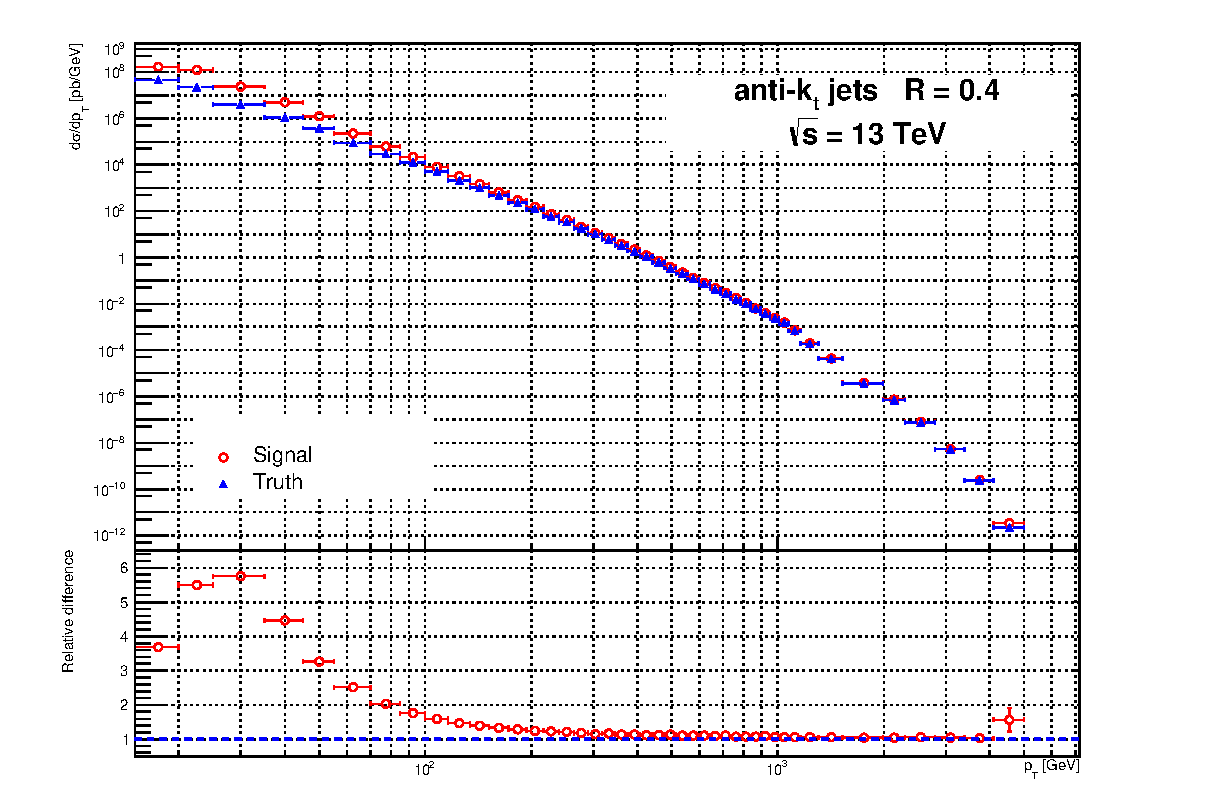
\includegraphics[width=0.8\textwidth]{{Chapter3/SignalVSTruth}.eps}
  \caption{Comparison of $\pt$ spectra of reco and truth jets after event
    selection. Each bin was divided by its width and all corresponding rapidity
    bins were merged to this histogram so $y$-axis has
    physical meaning of differential cross section in $\pt$.
    Bottom graph contains the relative difference between reco and truth
    differential cross section in $\pt$.} 
  \label{fig:SignalVSTruth}
\end{figure}

\section{Unfolding}
\label{Sec:Unfolding3}

Summarizing the results of the previous section, firstly the series of four
cutoffs was done on all events saved in Monte Carlo simulated data and the sets
of jets denoted reco and truth jets were obtained. Both reco and truth jets
were split into two categories depending on successful matching - there is
correspondence $1:1$ between matched reco and matched truth jets. Reco jets,
which were not matched, formed the unmatched reco jets, and similarly a set of
unmatched truth jets was created. All these 6 sets of jets are needed by the
unfolding procedure which description follows in this section.

Figure \ref{fig:SignalVSTruth} shows the $\pt$ spectra of reco and truth jets.
It can be seen, that observed $\pt$ spectrum, represented by the reco jets,
differs from the $\pt$ spectrum theoretically expected which is represented by
the $\pt$ spectrum of truth jets. Unfolding should transform the observed $\pt$
spectrum to the spectrum theoretically expected. If this transformation would be
done on real data, it should ideally preserve additional structures, which are
presented in data, but not included by the theory.


The main ingredient for the unfolding procedure is the transfer matrix $A_{ij}$
which contains the number of reco jets in bin $i$ with a matched truth jet that
was generated in bin $j$ and describes thus the smearing effects of the
detector.  In this thesis the double binning \ref{eq:Binning} is used which
complicates the situation because the matched reco jet can simply migrate of the
transfer matrix from Figure \ref{fig:UnfoldingMatrixDetail}, when its rapidity
$|y|>0.5$ and when it was matched with truth jet with $|y|<0.5$ or vice versa.
Two ways of dealing with double binning are assumed in this thesis.

\begin{enumerate}
  \item \textbf{Simple unfolding}
    
    In this case, only those reco and truth jets was used in the transfer
    matrix, which were matched within the same rapidity bin. Remaining matched
    jets were added to the unmatched statistic. 8 transfer matrices $46 \times
    46$ is filled (one for each rapidity bin, $46$ = number of $\pt$ bins) and
    unfolding is done for each of these matrices separately. One of these
    matrices for $|y|<0.5$ rapidity bin is shown at Figure
    \ref{fig:UnfoldingMatrixDetail}.

  \item \textbf{2D unfolding}

    In this case, the unfolding matrix was redefined to encapsulate the matching
    of jets between two different rapidity bins. In this case only one transfer
    matrix $368 \times 368$ is created ($368 = 46 \cdot 8$) with unfolding being
    done only for this matrix shown at Figure \ref{fig:UnfoldingMatrixAll}, from which
    the way how the transfer matrix was redefined from the simple unfolding
    should follow.
\end{enumerate}

\begin{figure}[p]
  \centering
  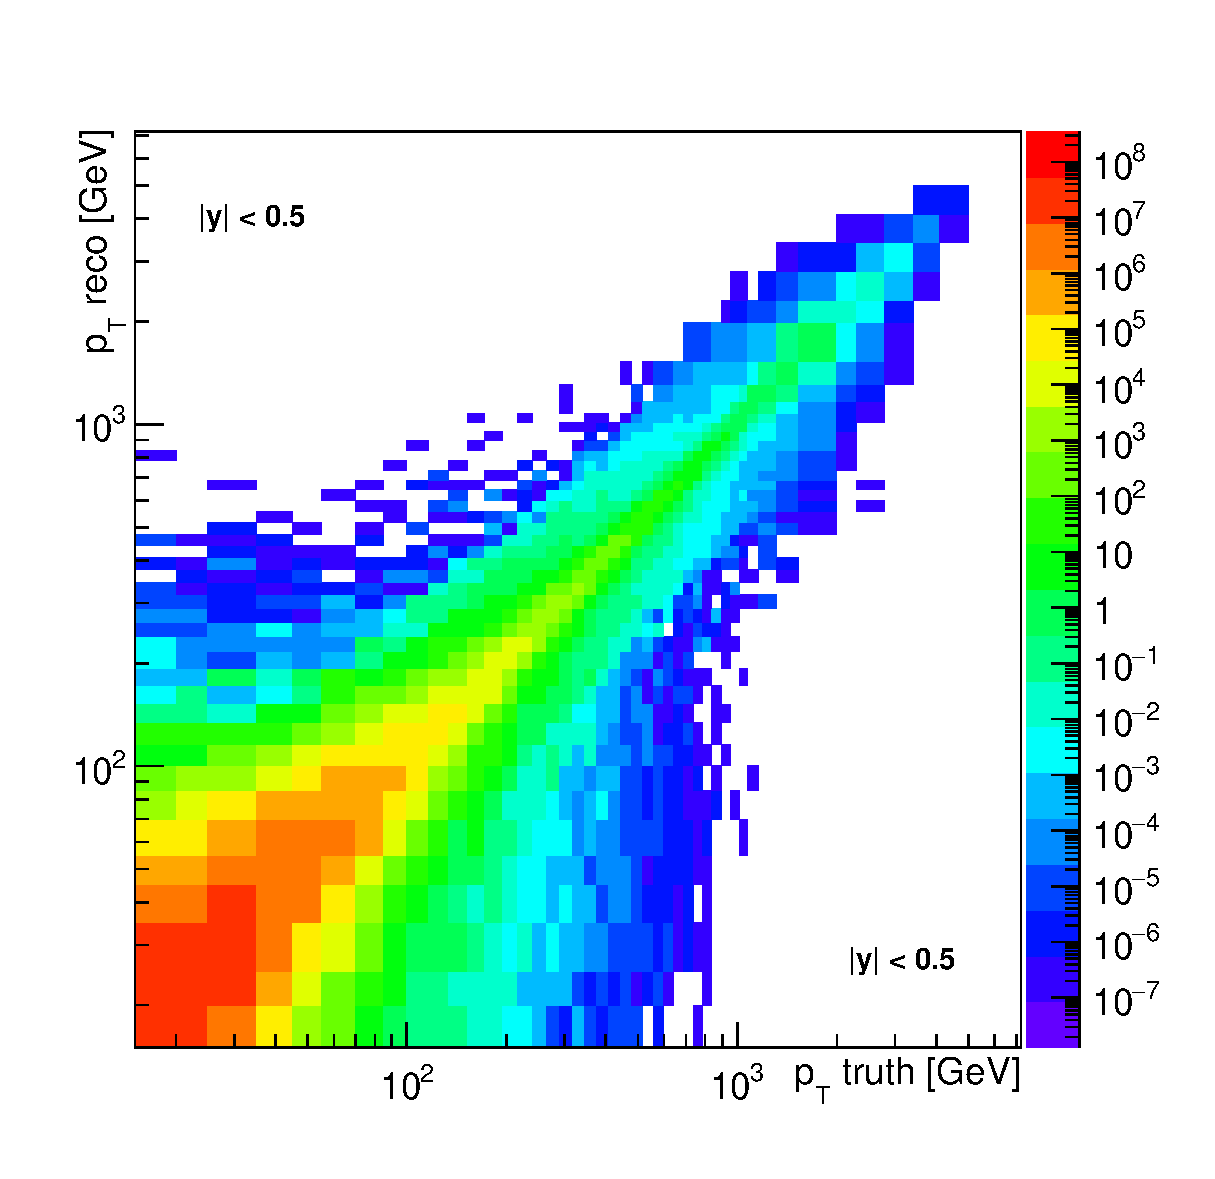
\includegraphics[width=\textwidth]{{Chapter3/Unfold_matrix_firstBin}.eps}
  \caption{Unfolding matrix for matched reco and truth jets with rapidity
  $|y|<0.5$ corresponding to one of eight matrices used in the simple unfolding.
  Each cell is proportional to the number of jets with truth $\pt$ in range
  determined by the $x$-axis which were reconstructed to the reco jets
  with $\pt$ determined by the $y$-axis. White space signalize no input.}
  \label{fig:UnfoldingMatrixDetail}
\end{figure}

\begin{figure}[p]
  \centering
  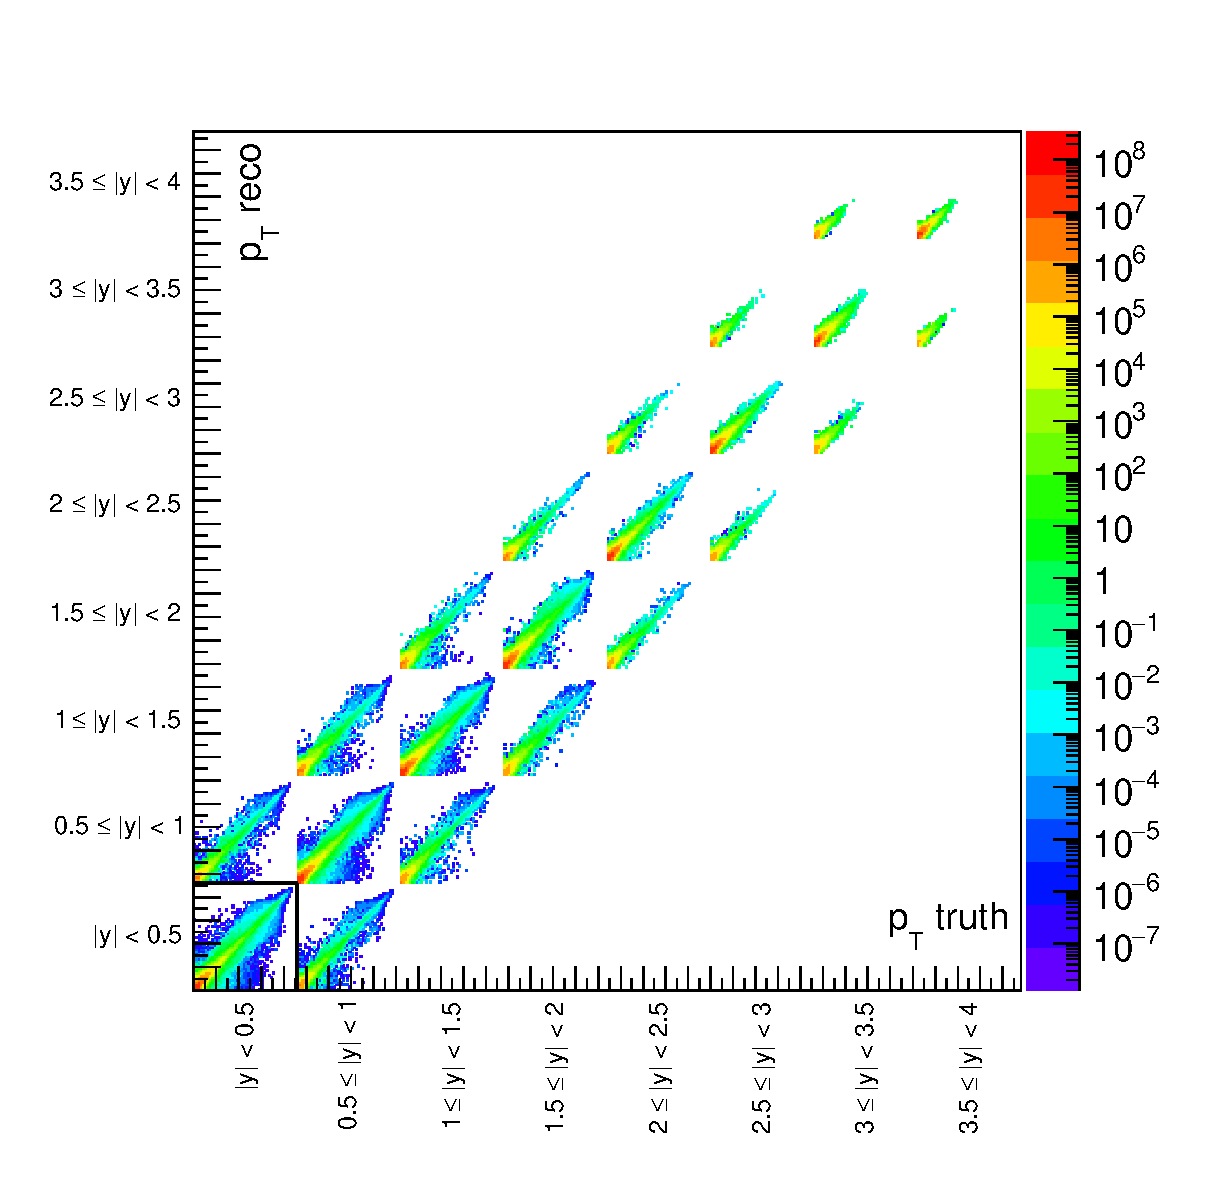
\includegraphics[width=\textwidth]{{Chapter3/Unfold_matrix_all}.eps}
  \caption{Unfolding matrix used in the 2D unfolding. Each cell is
    proportional to the number of jets with truth $\pt$ and rapidity $y$
    determined by the $x$-axis, which were reconstructed to the reco jets with
    $\pt$ and $y$ determined by the $y$-axis. Marked square in $|y|<0.5$ region
    is the matrix shown in Figure \ref{fig:UnfoldingMatrixDetail}. Projection of
    this matrix on the $x$ and $y$-axis corresponds to the $\pt$ spectrum of
    matched truth and reco jets for corresponding rapidity bin respectively.}
  \label{fig:UnfoldingMatrixAll}
\end{figure}

Transfer matrix from Figure \ref{fig:UnfoldingMatrixAll} used by the 2D
unfolding contains at the diagonal 8 submatrices which are the unfolding
matrices used by the simple unfolding. Next to these diagonal submatrices
transfer matrix of 2D unfolding contains 14 additional submatrices beside
diagonal. These corresponds to the matched jets with migration in rapidity bins
and in case of simple unfolding, these jets are assumed to be unmatched.

Dominant elements of each of the submatrices are on the main diagonal, which
corresponds to the fact, there is no significant bias in $\pt$ reconstruction.
The finite $\pt$ resolution causes the smearing of the diagonal and finite
rapidity resolution is the cause of the 14 minor submatrices.

Next to the transfer matrix, numbers of matched and unmatched reco and truth
jets are needed for each $(y,\pt)$ bin by unfolding procedure. These serve for
calculation of matching efficiency which is the key ingredient in the first and
the last step of unfolding procedure. Matching efficiencies for $|y|<0.5$
rapidity bin are for both simple and 2D unfolding shown at Figure
\ref{fig:MatchingEfficiencyDemonstration} and for other rapidity bins, the
results are shown in Appendix \ref{sec:MatchingEfficiency}

\begin{figure}[p]
  \centering
  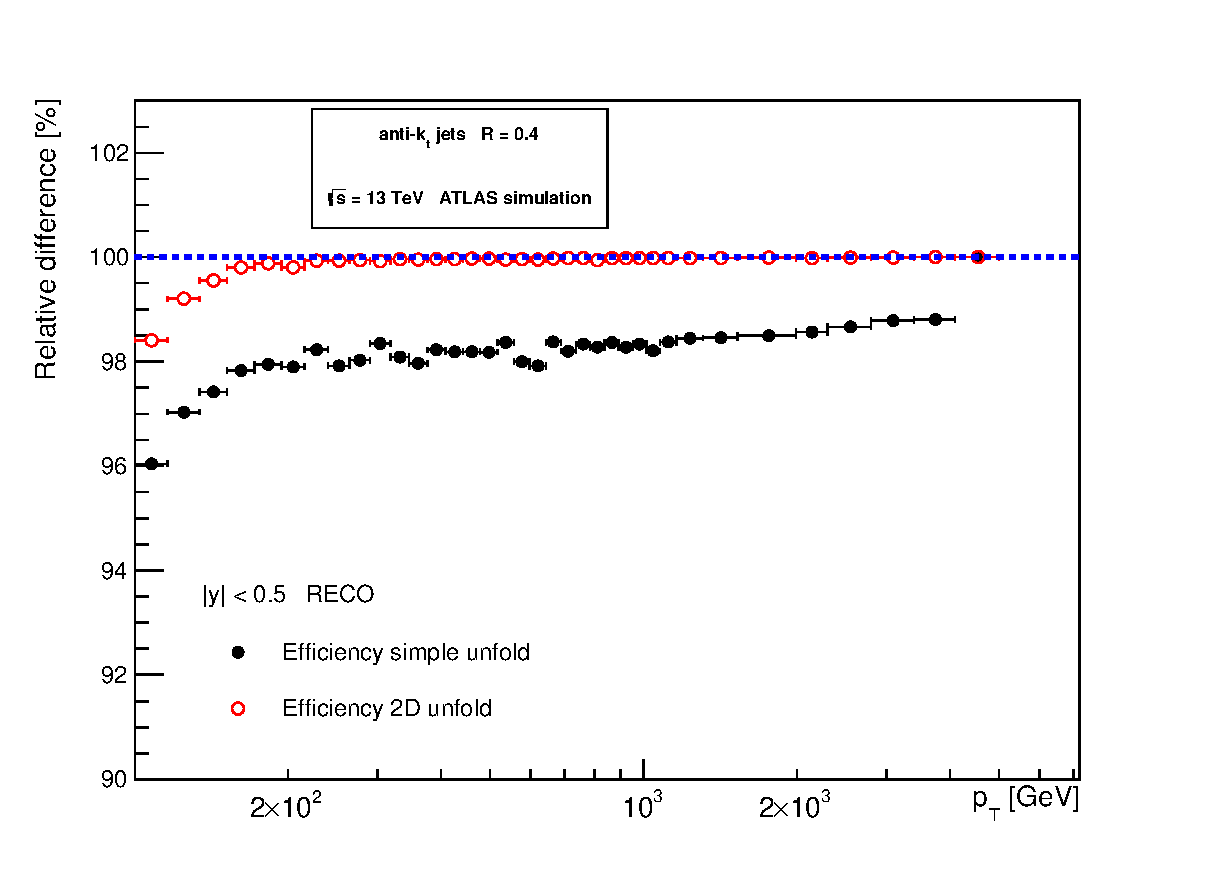
\includegraphics[width=0.49\textwidth]{{Chapter3/MatchEffSimpe2DSignal|abs(y)|0-0.5Compare}.eps}
  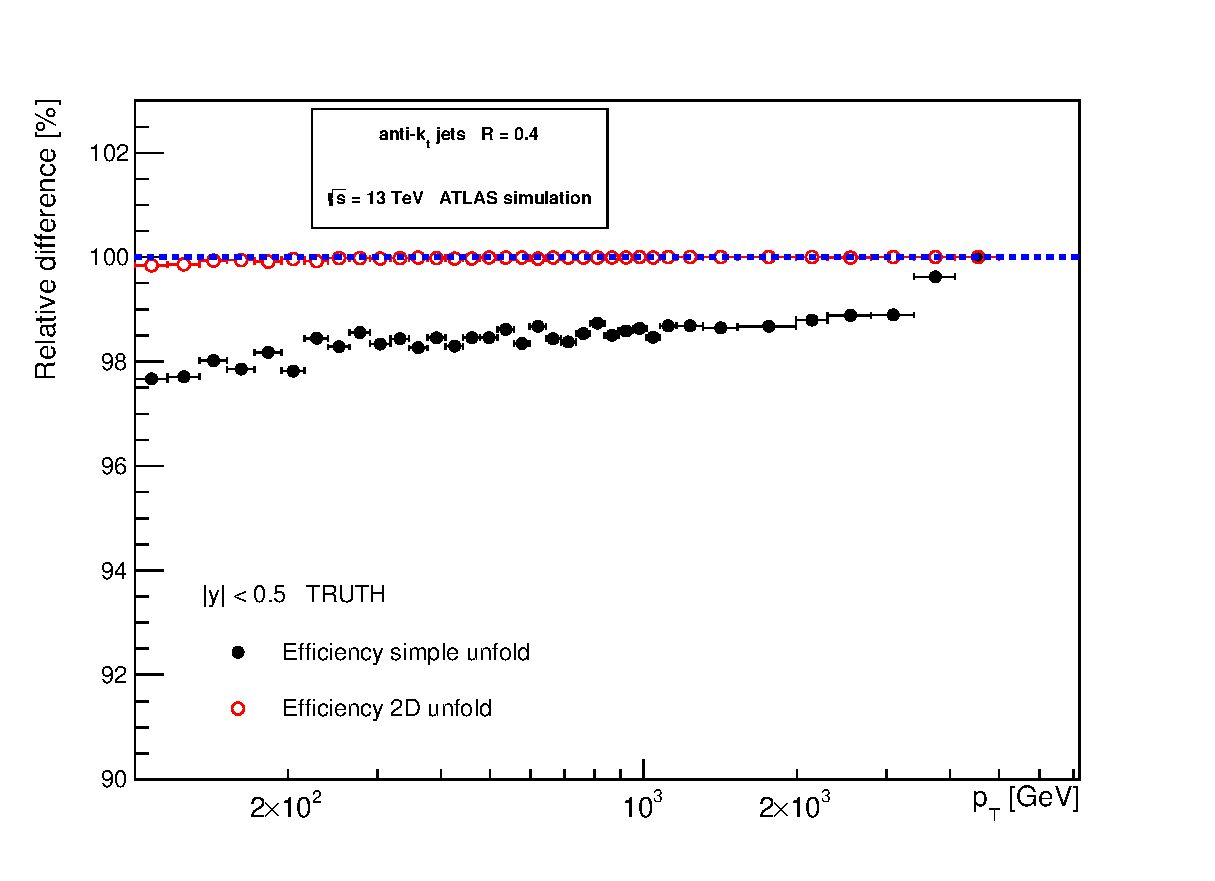
\includegraphics[width=0.49\textwidth]{{Chapter3/MatchEffSimpe2DTruth|abs(y)|0-0.5Compare}.eps}
  \caption{Comparison of matching efficiency of simple and 2D unfolding for $|y|
    < 0.5$ rapidity bin. Matching efficiency is compared for both reco jets
    (left) and truth jets (right). Matching efficiency for all rapidity bins is
    shown in Appendix \ref{sec:MatchingEfficiency}.}
  \label{fig:MatchingEfficiencyDemonstration}

  \vspace{1cm}

  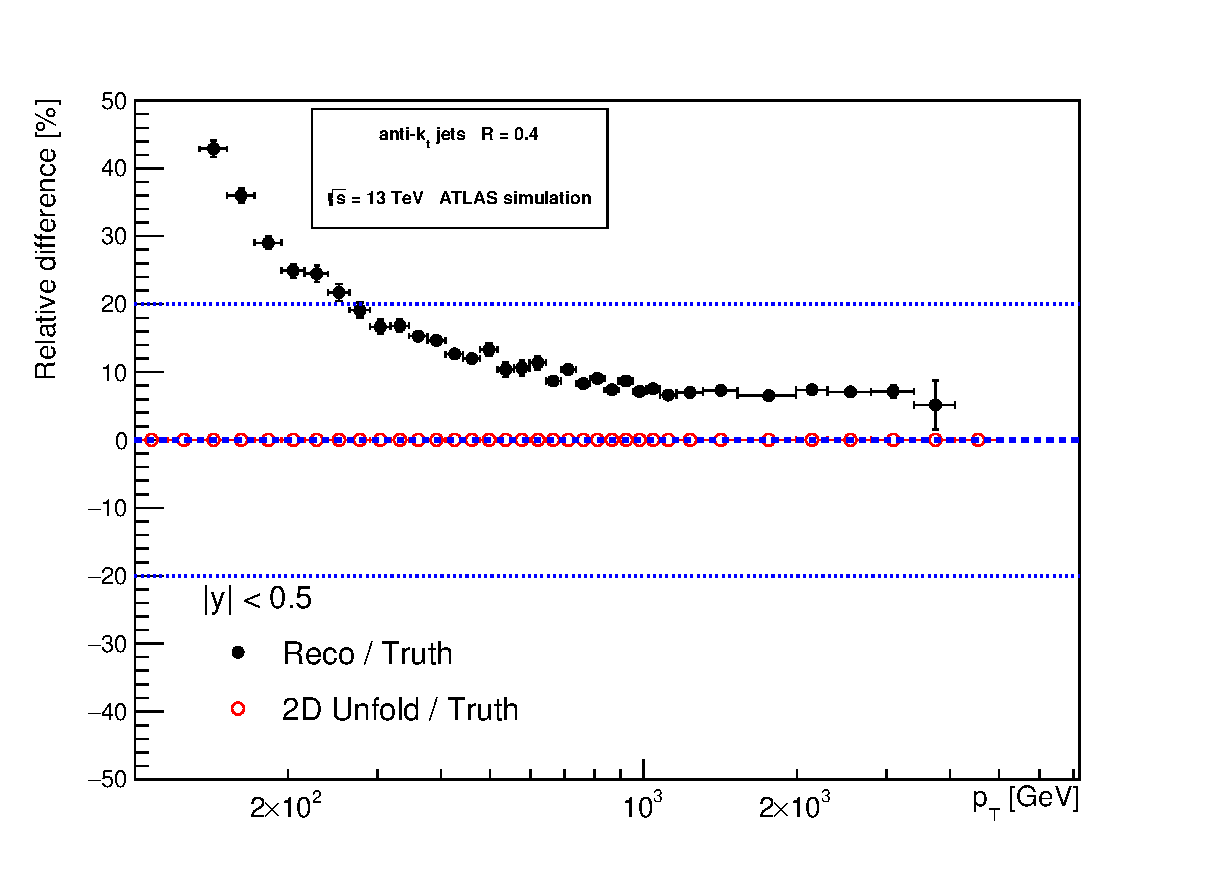
\includegraphics[width=0.49\textwidth]{{Chapter3/SignalUnfolded_VS_Truth|abs(y)|0-0.5Compare}.eps}
  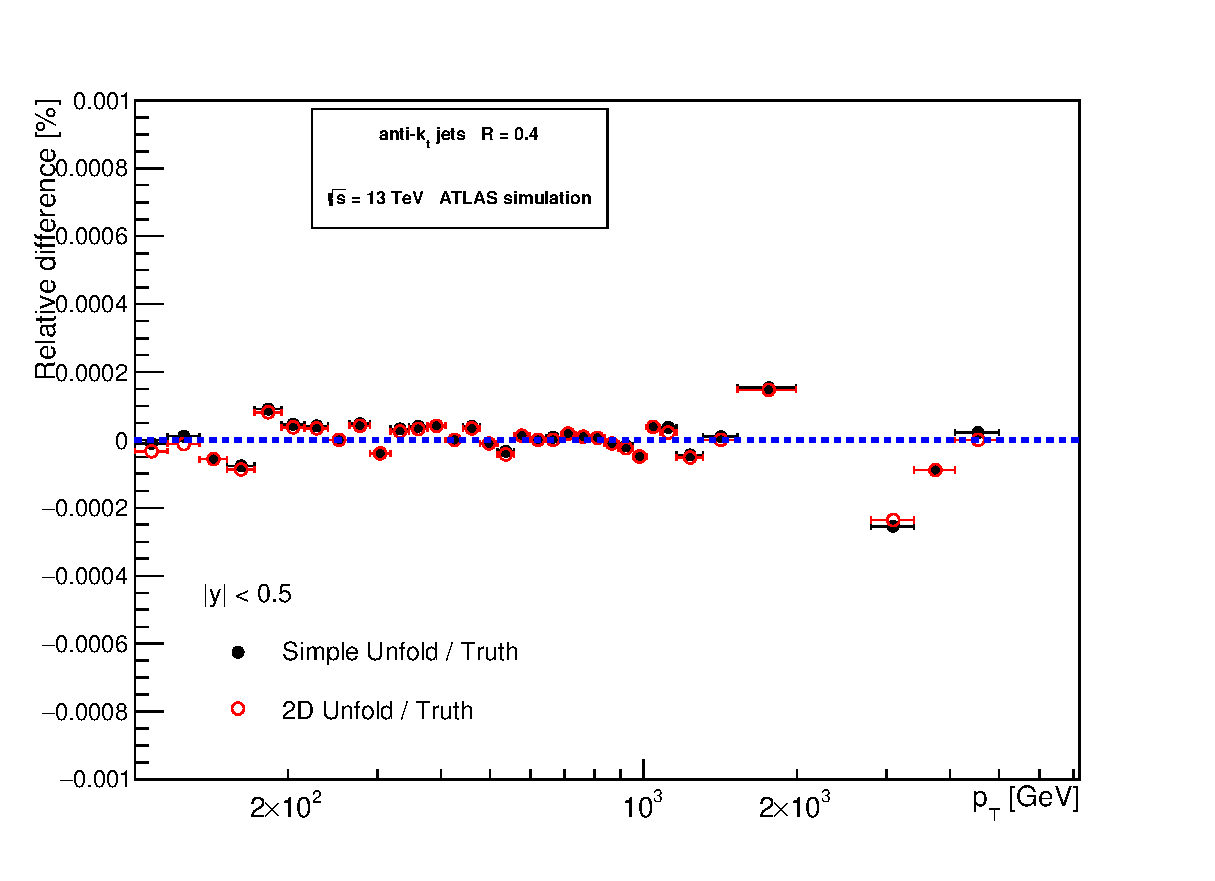
\includegraphics[width=0.49\textwidth]{{Chapter3/UnfoldedSimpleComplex_VS_Truth|abs(y)|0-0.5Compare}.eps}
  \caption{Comparison of $\pt$ spectra of signal jets and the unfolded
    $\pt$ spectra (2D unfolding) with the $\pt$ spectra of the truth jets
    (left). Comparison of unfolded spectra obtained by the 2D and simple
    unfolding with the $\pt$ spectra of the truth jets (right). Both graphs are
    for $|y|<0.5$ rapidity regions. Results for all rapidity bins are shown in
    Appendices \ref{sec:UnfoldingResults}, \ref{sec:SimpleAnd2DUnfolding}. }
  \label{fig:UnfoldingResultsDemonstration}
\end{figure}


Unfolding procedure can be divided into three main steps

\begin{enumerate}
  \item Input data are multiplied by the matching efficiency of signal jets.
  \item Transfer matrix is used to correct data spectrum for detector effects.
    For this purpose, the Iterative Dynamical Stabilized (IDS)
    \cite{IterativeDynamicallyStabilized} unfolding method was used which uses
    the series of iterations to improve unfolding results. In this thesis the
    iteration was done once.
  \item Spectrum obtained by the step 2 is divided by the matching efficiency of
    truth jets in order to correct resulting spectrum for the unmatched truth
    jets.
\end{enumerate}

Figure \ref{fig:UnfoldingResultsDemonstration} shows the comparison of $\pt$
spectra of signal jets and unfolded spectrum (by 2D unfolding method) with the
$\pt$ spectrum of truth jets (left) and the comparison of simple and 2D unfolded
spectra with the spectrum of truth jets (right) for $|y|<0.5$ rapidity bin.
Results for all rapidity bins are shown in Appendix \ref{sec:UnfoldingResults}.

From figures it follows, the unfolding procedure corrects the
$\pt$ spectrum of reco jets to $\pt$ spectrum of truth jets up to the systematic
error $<10^{-3}\,\%$ and that the differences between results of simple and 2D
unfolding are even smaller.

\section{Comparison with NLO Prediction}

The unfolded $\pt$ spectrum obtained in the previous section, was compared with
the $\pt$ spectrum obtained by the NLO QCD calculations.  These calculations was
done with \textsc{NLOJET++} program v4.1.2 \cite{NLOJetProgram} using CT10 NLO PDF set
\cite{CT10PDF}.

NLO predictions were compared for two different center-of-mass energies of $pp$
collisions - first corresponding to the LHC Run I ($\sqrt{s}=8\TeV$) and second
to Run II ($\sqrt{s} = 13\TeV$).  This comparison is shown for $|y|<0.5$
rapidity bin in Figure \ref{fig:ComparePredictionsDemonstation}, where also the
differential cross section is multiplied by the $\pt$ bin width and by
the integrated luminosity of Run I ($20\,\text{fb}^{-1}$) and expected
integrated luminosity of Run II ($100\,\text{fb}^{-1}$) to obtain expected number
of jets observed in each $\pt$ bin. Comparisons for other rapidity bins are
shown in Appendix \ref{sec:PredictionsForRunIAndII}.

\begin{figure}[t]
  \centering
  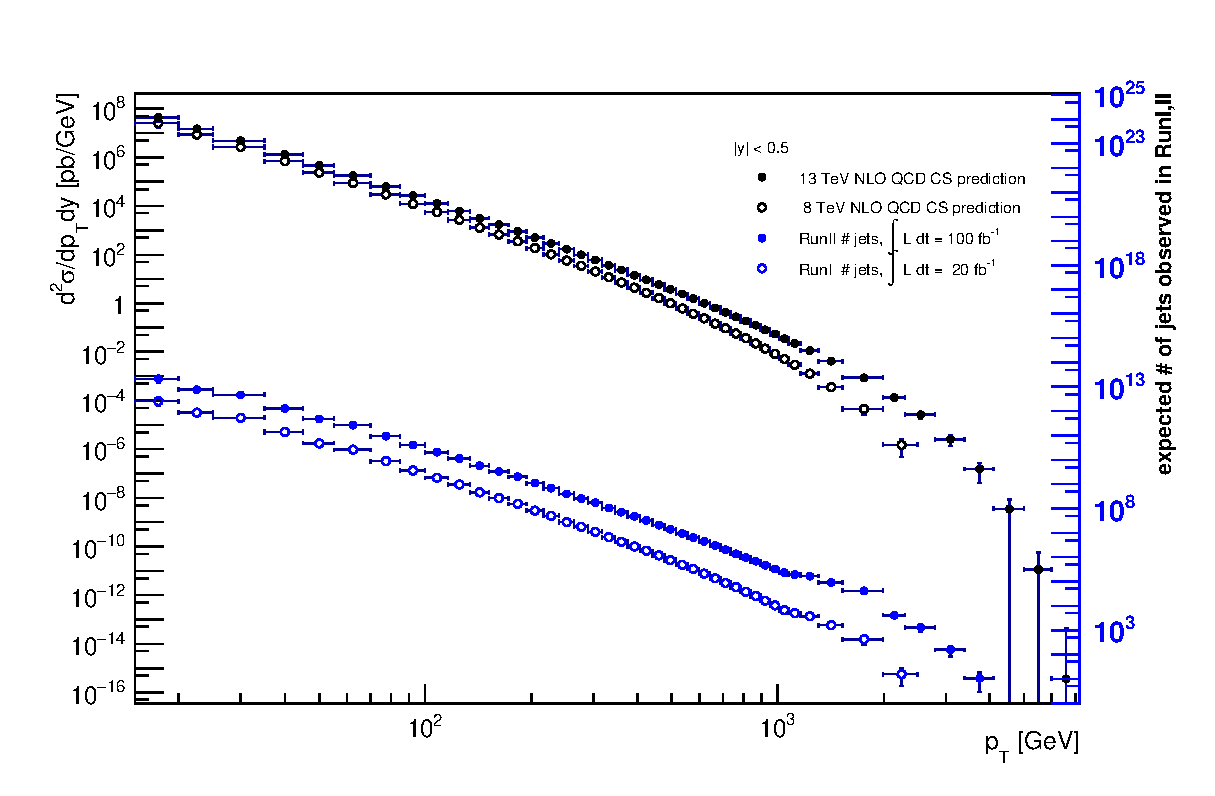
\includegraphics[width=0.8\textwidth]{{Chapter3/PredictionCompare0}.eps}
  \caption{Comparison of NLO QCD prediction of double differential inclusive jet
    cross section (black) for $pp$ collisions at $\sqrt{s}=13\TeV$ (filled circles)
    corresponding to the LHC Run II and $\sqrt{s}=8\TeV$ (empty circles)
    corresponding to the LHC Run I. The cross section is multiplied by
    integrated luminosities and $\pt$ bin width to obtain the expected number of jets
    observed in each $\pt$ bin (blue). Figure shows only $|y|<0.5$ rapidity bin,
    remaining rapidity bins are shown in Appendix \ref{sec:PredictionsForRunIAndII}.}
  \label{fig:ComparePredictionsDemonstation}
\end{figure}

It can be seen, that the increase in the center-of-mass energy is the most
significant for jets with high $\pt$. By the NLO QCD theoretical computations, several
uncertainties are taken into account. These include \cite{Analysis2012}

\begin{itemize}
  \item \textbf{Scale uncertainty}

    Coming from the choice of renormalization and factorization scales,
    including neglecting the higher order terms beyond NLO and making choice in
    scale, where the hard processes are replaced by hadronisation. 

  \item \textbf{$\alpha_S$ uncertainty}

    Because $\alpha_S$ is experimentally determined with error as is shown in
    Figure with running coupling constant \ref{fig:RunningCouplingConstant}.

  \item \textbf{PDF uncertainty}

    Prediction depends on the concrete choice of PDF.

  \item \textbf{Nonperturbative corrections uncertainty}

    ???

  \item \textbf{Electroweak corrections uncertainty}

    Next to the QCD processes, the electroweak processes has to be assumed.
    These processes becomes more important, as the momentum transfer increases.
\end{itemize}

In this analysis, only first three of these corrections are assumed. The
corrections were extracted from the files with NLO QCD predictions, where each
correction is represented by the set of equally likely histograms differing
from the default prediction. Correction was determined as the square sum of all
the corrections up and down separately and for $|y|<0.5$ rapidity bin are shown
at Figure \ref{fig:NLOSystematicsDemonstartion}, other rapidity bins are shown
in Appendix \ref{sec:NLOUncertainties}.

\begin{figure}[p]
  \centering
  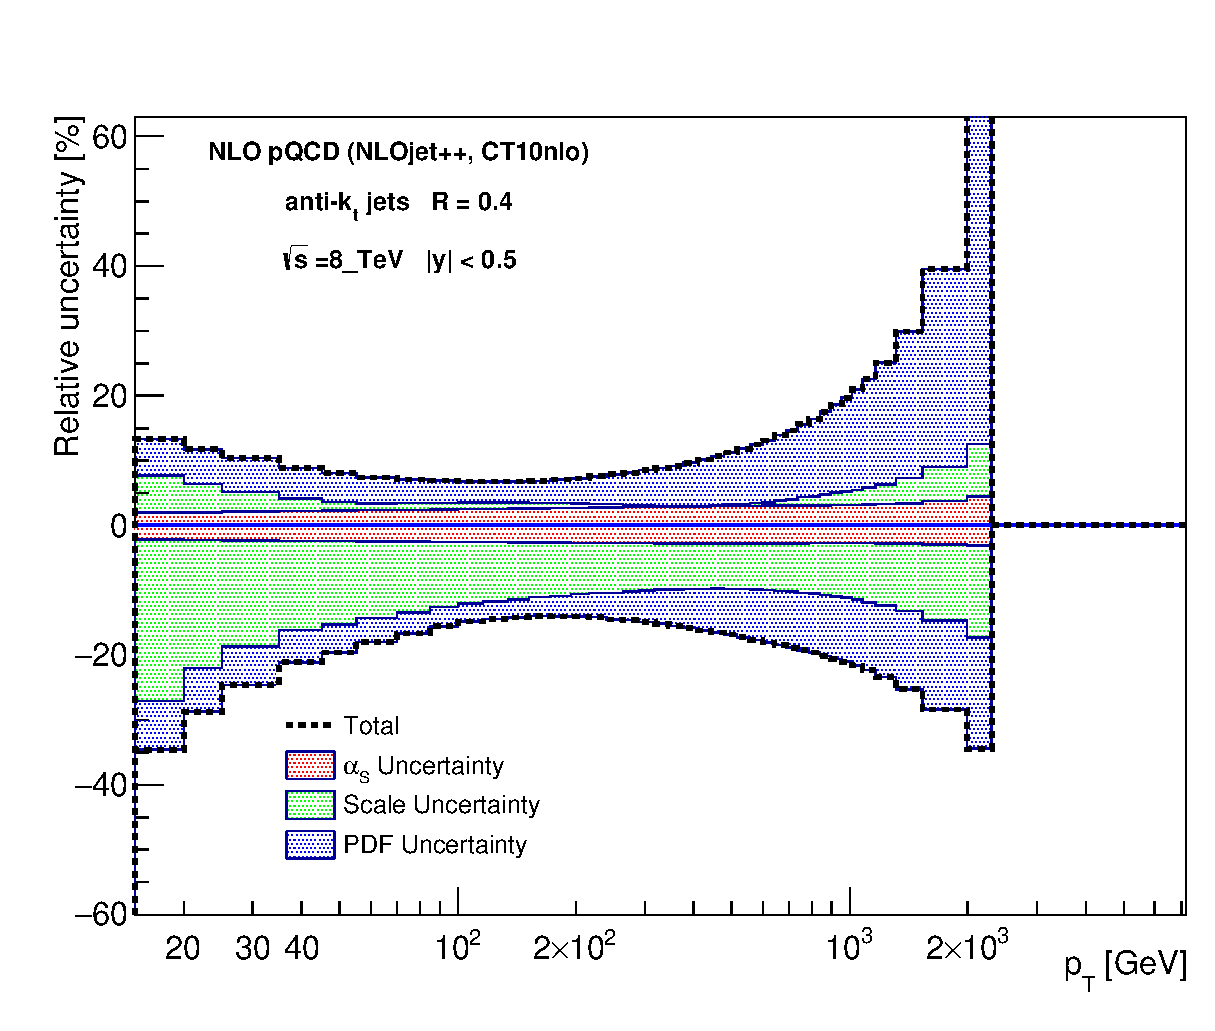
\includegraphics[width=0.49\textwidth]{{Chapter3/NLO_Systematics8_TeV0}.eps}
  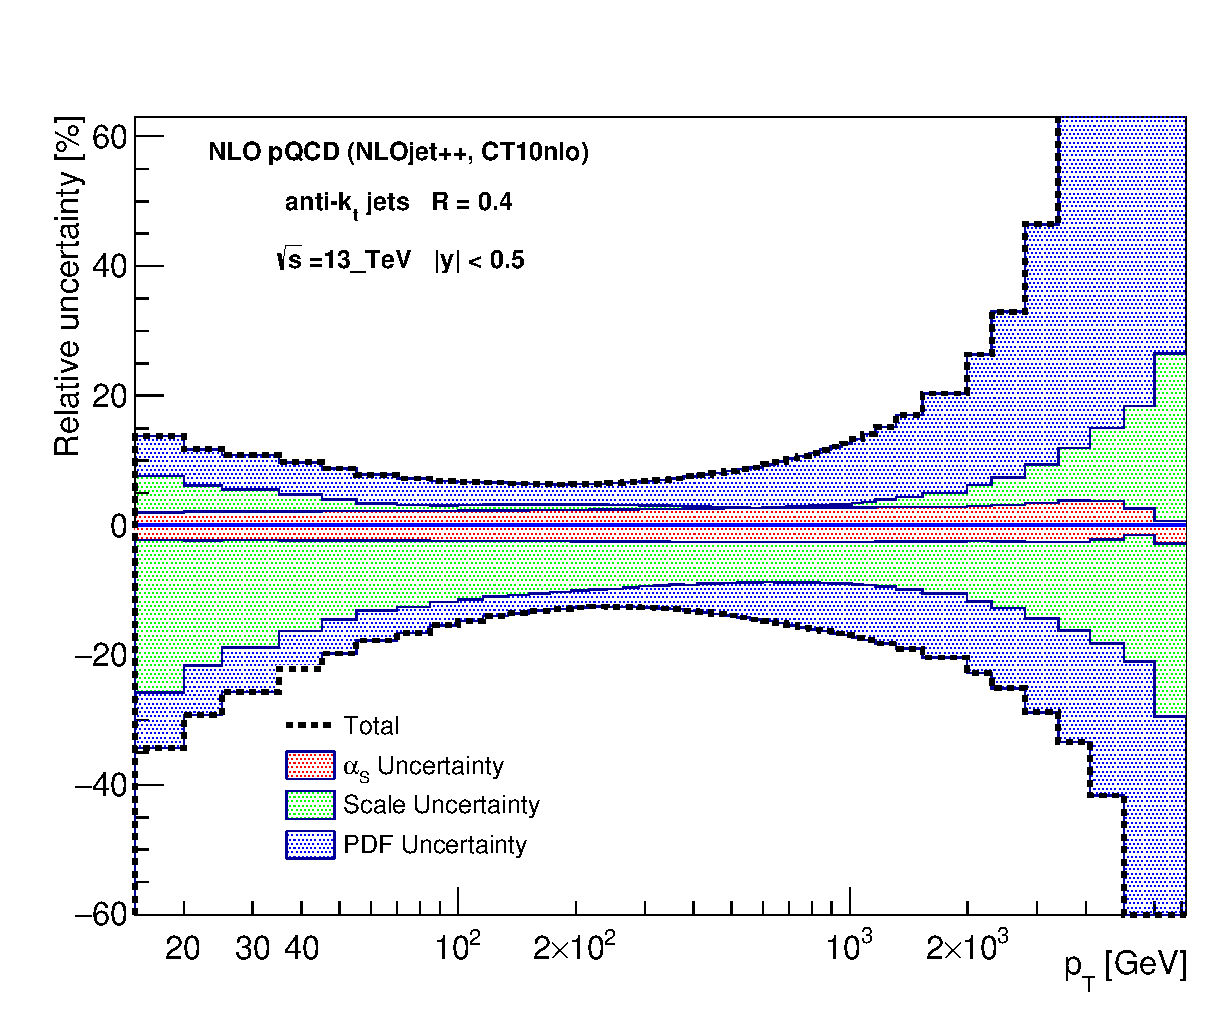
\includegraphics[width=0.49\textwidth]{{Chapter3/NLO_Systematics13_TeV0}.eps}
  \caption{NLO uncertainties for NLO QCD predictions of inclusive jet
    differential cross section for $pp$ collisions at
    $\sqrt{s}=8\TeV$ (left) and $\sqrt{s}=13\TeV$ (right) for $|y|<0.5$ rapidity
    bin. Uncertainties for other rapidity bins are shown in Appendix
    \ref{sec:NLOUncertainties}.}
  \label{fig:NLOSystematicsDemonstartion}

  \vspace{1cm}

  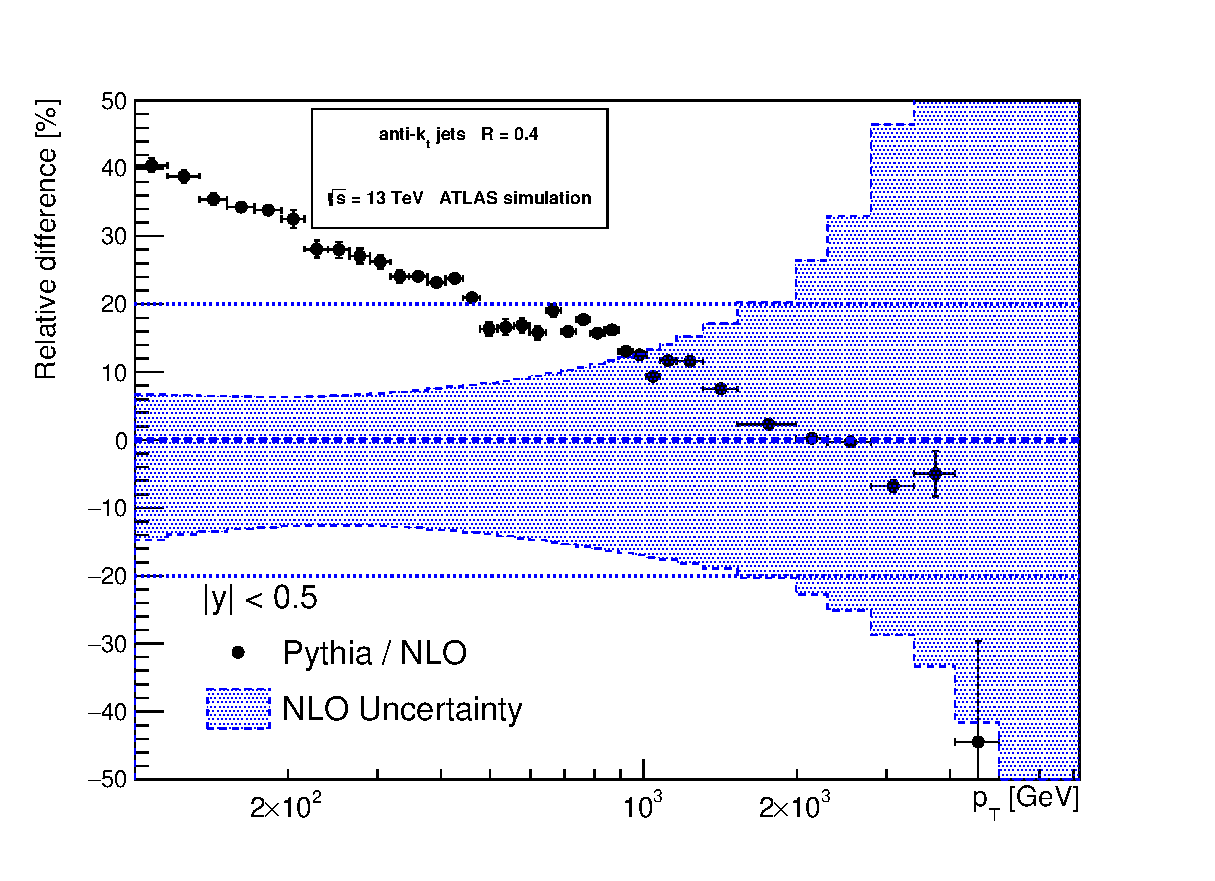
\includegraphics[width=0.8\textwidth]{{Chapter3/Truth_VS_Prediction|abs(y)|0-0.5Compare}.eps}
  \caption{Comparison of \textsc{Pythia8} prediction with NLO QCD prediction of
    inclusive jet double differential cross section for $|y|<0.5$ rapidity bin
    with uncertaintis of NLO QCD predictions symbolized by the blue area.
    Comparisons for other rapidity bins are shown in Appendix
    \ref{sec:PythiaAndNLO}.}
  \label{fig:TruthVSPredictionsDemonstation}
\end{figure}

Comparison of $\pt$ spectra of truth jets with NLO QCD prediction is for $|y| <
0.5$ rapidity bin shown at Figure \ref{fig:TruthVSPredictionsDemonstation} for
other rapidity bins see Appendix \ref{sec:PythiaAndNLO}.
